\documentclass[conference]{IEEEtran}
\usepackage{amsmath,amssymb,amsthm}
\usepackage{graphicx}
\usepackage{booktabs}
\usepackage{cite}
\usepackage[hidelinks]{hyperref}
\graphicspath{{figures/}}
\pdfminorversion=4

\newtheorem{proposition}{Proposition}
\newcommand{\bv}[1]{\mathbf{#1}}
\newcommand{\Jm}{\boldsymbol{\mathcal{J}}}

\begin{document}

\title{Flatness-Based and Passivity-Based Control with Adaptive Neural Compensation of a Direct-Drive PMSG Wind Energy Conversion System}

\author{
\IEEEauthorblockN{Said Regani}
\IEEEauthorblockA{\textit{L2EI Laboratory}\\
\textit{Jijel University}\\
BP 98 Ouled Aissa, Jijel 18000, Algeria}
\and
\IEEEauthorblockN{Manal Messadi}
\IEEEauthorblockA{\textit{L2EI Laboratory}\\
\textit{Jijel University}\\
BP 98 Ouled Aissa, Jijel 18000, Algeria}
\and
\IEEEauthorblockN{Kemih Karim}
\IEEEauthorblockA{\textit{L2EI Laboratory}\\
\textit{Jijel University}\\
BP 98 Ouled Aissa, Jijel 18000, Algeria}
}

\maketitle

\begin{abstract}
This paper presents the modeling and control of a grid-connected 2~MW direct-drive permanent magnet
synchronous generator (PMSG) wind turbine with a back-to-back converter and an $L$ filter. The model is
written in the receptor convention and its signs are verified by an exact power balance. The rotor
speed and the energy stored in the DC link and in the filter are used as flat outputs of the two outer
loops, and the current loops of both converters are designed by passivity-based control (PBC). A radial
basis function (RBF) network, adapted online by a Lyapunov law with $\sigma$-modification, learns the
uncertainty of the aerodynamic-torque model and of the generator parameters, and its stability is
proven. Simulations over 40~s with turbulent wind, parameter mismatch and a 50\,\% grid voltage dip
show that, compared with PI vector control tuned on the same poles, the proposed control reduces the
speed tracking error by 24\,\% and keeps the DC-link voltage within
0.21~V outside the dip (against 9.9~V), while the network reduces the speed
error by a further 35\,\%. The energy captured is the same for all controllers
(MPPT efficiency 97.7\,\%).
\end{abstract}

\begin{IEEEkeywords}
PMSG, wind energy conversion, flatness, passivity-based control, RBF neural network, back-to-back converter.
\end{IEEEkeywords}

\section{Introduction}
Wind energy is one of the main sources in the transition towards low-carbon electricity
generation~\cite{iea2024,gwec2024}. Direct-drive PMSG turbines remove the gearbox, which reduces
maintenance and losses, and their full-scale back-to-back converter decouples the generator from the
grid~\cite{polinder2013,wu2011}. The converter must track the maximum power point, regulate the DC-link
voltage and inject the power into the grid at unity power factor.

These tasks are usually performed by cascaded PI loops in rotating frames~\cite{chinchilla2006,yazdani2010}.
The PMSG model is nonlinear and coupled, the aerodynamic torque is not measured, and the parameters vary
with temperature and saturation. Nonlinear controllers have therefore been studied for wind turbines
and PMSGs, such as backstepping~\cite{mechter2016}, predictive control~\cite{messadi2015} and
passivity-based control~\cite{takhi2020}. Differential flatness~\cite{fliess1995} computes the control
directly from the desired trajectory of a flat output; with the stored energy as flat output, the DC-link
dynamics become a linear power balance~\cite{thounthong2010}. Passivity-based control~\cite{ortega1998}
shapes the energy of the closed loop and keeps the workless coupling terms of the machine. Both methods
use a model: their weak point is the uncertain aerodynamic torque, which neural networks can learn
online~\cite{lewis1999,regani2026}.

This paper applies these tools to the complete chain of a 2~MW direct-drive PMSG turbine:
\begin{itemize}
\item a model in the receptor convention whose signs are checked by an exact power balance;
\item flat outer loops for the rotor speed and for the energy of the DC link and filter, and PBC
current loops for both converters;
\item an RBF network that learns the aerodynamic-torque and parameter uncertainty inside the flat speed
law, with a Lyapunov stability proof;
\item an evaluation under turbulent wind, parameter mismatch and a grid voltage dip against PI vector
control tuned on the same poles.
\end{itemize}

\section{Wind Turbine Model}
The power captured by the rotor and its tip-speed ratio are~\cite{heier2014}
\begin{equation}
P_w = \tfrac{1}{2}\rho\pi R^2 C_p(\lambda,\beta)\,v^3,\qquad \lambda=\frac{\Omega R}{v}
\label{eq:pw}
\end{equation}
where $\rho$ is the air density, $R$ the rotor radius, $v$ the wind speed, $\Omega$ the rotor speed and
$\beta$ the pitch angle ($\beta=0$ below rated wind). The power coefficient is
\begin{equation}
C_p = 0.5176\Bigl(\frac{116}{\lambda_i}-0.4\beta-5\Bigr)e^{-21/\lambda_i}+0.0068\lambda,
\label{eq:cp}
\end{equation}
with $1/\lambda_i=1/(\lambda+0.08\beta)-0.035/(\beta^3+1)$; its maximum $C_{p,\max}=0.48$ is reached at
$\lambda_{opt}=8.1$. The aerodynamic torque is $T_w=P_w/\Omega$ and the direct-drive shaft obeys
\begin{equation}
J\frac{d\Omega}{dt} = T_w + T_e - B\Omega
\label{eq:shaft}
\end{equation}
where $J$ is the total inertia, $B$ the friction coefficient and $T_e$ the electromagnetic torque in the
receptor convention ($T_e<0$ in generating mode).

The wind speed combines a mean value, the low-frequency harmonics of~\cite{regani2026} and a turbulence:
\begin{equation}
v(t) = V_m + \textstyle\sum_{k=1}^{3} A_k\sin(2\pi f_k t) + v_t(t)
\label{eq:wind}
\end{equation}
with $V_m=8.5$~m/s, $A=[1.5,\,0.2,\,0.3]$~m/s and $f=[0.03,\,0.16,\,0.17]$~Hz. The rotor-effective
turbulence $v_t$ is a first-order coloured noise with standard deviation 0.5~m/s (6\,\% of $V_m$) and
correlation time 1.5~s. The wind used by the controller is measured by an anemometer modelled by a
first-order lag of 1~s, $v_m$.

\section{PMSG, Converters and Grid}
\subsection{PMSG}
In the rotor $dq$ frame (amplitude-invariant transformation, $d$ axis on the magnet flux), with the
receptor convention and $L_d=L_q=L_s$~\cite{wu2011},
\begin{align}
v_{sd} &= R_s i_{sd} + L_s\frac{di_{sd}}{dt} - \omega_e L_s i_{sq}\label{eq:vsd}\\
v_{sq} &= R_s i_{sq} + L_s\frac{di_{sq}}{dt} + \omega_e L_s i_{sd} + \omega_e\psi_f\label{eq:vsq}\\
T_e &= \tfrac32 p\,\psi_f\, i_{sq}\label{eq:te}
\end{align}
where $\omega_e=p\Omega$, $p$ is the number of pole pairs and $\psi_f$ the magnet flux. In generating mode
$i_{sq}<0$. With $\bv{i}_s=[i_{sd}\;i_{sq}]^T$, $\bv{v}_s=[v_{sd}\;v_{sq}]^T$, $\bv{e}_q=[0\;1]^T$ and
the skew-symmetric matrix $\Jm=\bigl[\begin{smallmatrix}0&1\\-1&0\end{smallmatrix}\bigr]$,
\begin{equation}
L_s\dot{\bv{i}}_s = \bv{v}_s - R_s\bv{i}_s + \omega_eL_s\Jm\bv{i}_s - \omega_e\psi_f\bv{e}_q .
\label{eq:pmsg}
\end{equation}

\subsection{Back-to-Back Converter, DC Link and Grid}
The two-level converters are represented by their average model; the voltage vectors are limited to
$V_{dc}/\sqrt3$ (space-vector modulation). The DC link receives the power of the machine-side converter
(MSC) and supplies the grid-side converter (GSC):
\begin{equation}
CV_{dc}\frac{dV_{dc}}{dt} = P_{dc} - P_i,\quad P_{dc}=-\tfrac32\bv{v}_s^T\bv{i}_s,\quad
P_i=\tfrac32\bv{v}_i^T\bv{i}_g .
\label{eq:dc}
\end{equation}
In the grid-voltage-oriented frame ($v_{gq}=0$, ideal PLL), the $L$ filter between the GSC voltage
$\bv{v}_i$ and the grid voltage $\bv{v}_g$, with the current $\bv{i}_g$ counted towards the grid, gives
\begin{equation}
L_f\dot{\bv{i}}_g = \bv{v}_i - R_f\bv{i}_g + \omega_gL_f\Jm\bv{i}_g - \bv{v}_g ,
\label{eq:filter}
\end{equation}
and the grid powers are $P_g=\frac32v_{gd}i_{gd}$ and $Q_g=-\frac32v_{gd}i_{gq}$.

\subsection{Power Balance}
Equations (\ref{eq:shaft}), (\ref{eq:pmsg})--(\ref{eq:filter}) form a sixth-order model with state
$[i_{sd},i_{sq},\Omega,V_{dc},i_{gd},i_{gq}]$. With the stored energy
$E=\frac12J\Omega^2+\frac34L_s\|\bv{i}_s\|^2+\frac12CV_{dc}^2+\frac34L_f\|\bv{i}_g\|^2$, and since
$\bv{x}^T\Jm\bv{x}=0$ and $T_e\Omega=\frac32\omega_e\psi_fi_{sq}$, the model gives exactly
\begin{equation}
\dot E = P_w - B\Omega^2 - \tfrac32R_s\|\bv{i}_s\|^2 - \tfrac32R_f\|\bv{i}_g\|^2 - P_g
\label{eq:balance}
\end{equation}
for any state and converter voltages: the aerodynamic power is stored, dissipated or delivered to the
grid. This identity checks every sign of the model; numerically, its residual is below
$10^{-15}P_n$.

Table~\ref{tab:param} lists the parameters. The turbine data ($R$, $\Omega_n$, $T_n$) correspond to a
2~MW direct-drive turbine; the generator, DC-link, filter and grid data are those of the non-salient
PMSG of~\cite{hasan2021}. The inertia gives an inertia constant $H=J\Omega_n^2/(2P_n)=3.5$~s. At the
rated point ($i_{sq}=-2.51$~kA, $\omega_e=58$~rad/s), the MSC voltage is 577~V and the GSC voltage
579~V, below the limit $V_{dc}/\sqrt3=693$~V.

\begin{table}[t]
\caption{Parameters of the Studied System}
\label{tab:param}
\centering
\footnotesize
\setlength{\tabcolsep}{4pt}
\begin{tabular}{llll}
\toprule
Parameter & Value & Parameter & Value\\
\midrule
$P_n$ & 2 MW & $p$ & 26\\
$R$ & 40 m & $R_s$ & 0.78 m$\Omega$\\
$\Omega_n$, $v_n$ & 2.23 rad/s, 11.0 m/s & $L_s$ & 1.57 mH\\
$T_n$ & 0.897 MN$\cdot$m & $\psi_f$ & 9.18 Wb\\
$\lambda_{opt}$, $C_{p,\max}$ & 8.1, 0.48 & $C$, $V_{dc}^*$ & 20 mF, 1200 V\\
$J$ & $2.8\times10^6$ kg$\cdot$m$^2$ & $L_f$, $R_f$ & 0.15 mH, 2 m$\Omega$\\
$B$ & $10^3$ N$\cdot$m$\cdot$s/rad & Grid & 690 V, 50 Hz\\
$\rho$ & 1.225 kg/m$^3$ & $f_{sw}$ & 2160 Hz\\
\bottomrule
\end{tabular}
\end{table}

\section{Proposed Control}
The structure is shown in Fig.~\ref{fig:structure}. All errors are defined as measured minus reference
values. The controller is sampled at $T_s=1/(2f_{sw})=231.5~\mu$s (regular sampling, double update).

\begin{figure}[t]
\centering
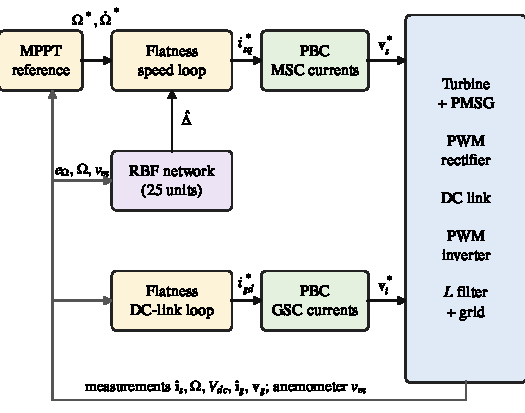
\includegraphics[width=0.92\columnwidth]{structure.pdf}
\caption{Control structure: flat outer loops, PBC current loops and RBF compensation.}
\label{fig:structure}
\end{figure}

\subsection{Speed Reference}
The optimal speed $\Omega_{opt}=\lambda_{opt}v_m/R$, limited to $[0.5\Omega_n,\Omega_n]$, is filtered by
$\ddot\Omega^*=\omega_r^2(\Omega_{opt}-\Omega^*)-2\omega_r\dot\Omega^*$ ($\omega_r=1$~rad/s), which
provides a smooth reference $\Omega^*$ and its derivative.

\subsection{Flatness-Based Speed Loop}
A system is flat if its states and inputs are functions of a flat output and of a finite number of its
derivatives~\cite{fliess1995}. Flatness is used here for the two outer subsystems, with the currents as
inputs. From (\ref{eq:shaft}), $T_e=J\dot\Omega+B\Omega-T_w$: $\Omega$ is a flat output of the shaft with
input $T_e$, i.e., $i_{sq}$. Imposing $\dot\Omega=\nu_1$ with
$\nu_1=\dot\Omega^*-k_{11}e_\Omega-k_{12}\!\int\!e_\Omega dt$, $e_\Omega=\Omega-\Omega^*$, gives
\begin{equation}
T_e^* = J\nu_1 + B\Omega - \hat T_w - \hat\Delta,\qquad i_{sq}^*=\frac{T_e^*}{\frac32p\psi_f},\quad i_{sd}^*=0
\label{eq:flat1}
\end{equation}
where $\hat T_w$ is the aerodynamic torque computed from (\ref{eq:pw})--(\ref{eq:cp}) with $v_m$ and
$\hat\Delta$ is the neural compensation (Section~IV-E). $T_e^*$ is limited to $[-1.2T_n,0]$ and the
integral is frozen at the limit. With $i_{sq}=i_{sq}^*$ and $\Delta=T_w-\hat T_w$,
\begin{equation}
J\bigl(\dot e_\Omega + k_{11}e_\Omega + k_{12}\!\textstyle\int\! e_\Omega dt\bigr) = \Delta-\hat\Delta .
\label{eq:errw}
\end{equation}

\subsection{Flatness-Based DC-Link Loop}
The flat output is the energy stored in the DC link and in the filter,
$y_2=\frac12CV_{dc}^2+\frac34L_f\|\bv{i}_g\|^2$. From (\ref{eq:dc})--(\ref{eq:filter}),
\begin{equation}
\dot y_2 = P_{dc} - P_g - \tfrac32R_f\|\bv{i}_g\|^2
\label{eq:y2}
\end{equation}
which is linear in the grid power~\cite{thounthong2010}; $V_{dc}$ follows from $y_2$ and the measured
currents, and $P_g$ from $\dot y_2$. Imposing $\dot y_2=-k_{21}e_y-k_{22}\int e_y\,dt$, with
$e_y=y_2-y_2^*$ and $y_2^*=\frac12CV_{dc}^{*2}+\frac34L_f\|\bv{i}_g^*\|^2$, gives
\begin{equation}
P_g^* = P_{dc} - \tfrac32R_f\|\bv{i}_g\|^2 + k_{21}e_y + k_{22}\!\int\! e_y dt,\quad
i_{gd}^*=\frac{2P_g^*}{3v_{gd}}
\label{eq:flat2}
\end{equation}
and $i_{gq}^*=-2Q_g^*/(3v_{gd})$ with $Q_g^*=0$. $P_{dc}$ is computed from the applied MSC voltages and
the measured currents, so the power coming from the generator is compensated before it changes
$V_{dc}$. The variation of $y_2^*$, due to the filter energy only (below 300~J against 14.4~kJ in the
capacitor), is neglected. The gains are $k_{11}=2\omega_\Omega$, $k_{12}=\omega_\Omega^2$,
$k_{21}=2\omega_v$, $k_{22}=\omega_v^2$ (Table~\ref{tab:ctrl}).

\subsection{Passivity-Based Current Loops}
With $\bv{e}_s=\bv{i}_s-\bv{i}_s^*$ and $\dot{\bv{z}}_s=\bv{e}_s$, the MSC voltage reference is
\begin{equation}
\bv{v}_s^* = L_s\dot{\bv{i}}_s^* + R_s\bv{i}_s^* - \omega_eL_s\Jm\bv{i}_s^* + \omega_e\psi_f\bv{e}_q
- R_a\bv{e}_s - K_i\bv{z}_s
\label{eq:pbc1}
\end{equation}
and, with $\bv{e}_g=\bv{i}_g-\bv{i}_g^*$ and $\dot{\bv{z}}_g=\bv{e}_g$, the GSC voltage reference is
\begin{equation}
\bv{v}_i^* = L_f\dot{\bv{i}}_g^* + R_f\bv{i}_g^* - \omega_gL_f\Jm\bv{i}_g^* + \bv{v}_g
- R_b\bv{e}_g - K_{ig}\bv{z}_g .
\label{eq:pbc2}
\end{equation}
The reference derivatives are obtained by first-order filters (2~ms); the integrals are frozen when the
voltage reaches $V_{dc}/\sqrt3$.

\begin{proposition}
With (\ref{eq:pbc1}) applied to (\ref{eq:pmsg}) and $R_a,K_i>0$, the storage function
$H=\frac12L_s\|\bv{e}_s\|^2+\frac12K_i\|\bv{z}_s\|^2$ satisfies $\dot H=-(R_s+R_a)\|\bv{e}_s\|^2$ and
$\bv{e}_s\to0$. The same holds for (\ref{eq:pbc2}) applied to (\ref{eq:filter}).
\end{proposition}
\begin{proof}
Subtracting $L_s\dot{\bv{i}}_s^*$ from (\ref{eq:pmsg}) and inserting (\ref{eq:pbc1}) gives
$L_s\dot{\bv{e}}_s=-(R_s+R_a)\bv{e}_s+\omega_eL_s\Jm\bv{e}_s-K_i\bv{z}_s$. Hence
$\dot H=\bv{e}_s^TL_s\dot{\bv{e}}_s+K_i\bv{z}_s^T\bv{e}_s=-(R_s+R_a)\|\bv{e}_s\|^2$, since
$\bv{e}_s^T\Jm\bv{e}_s=0$: the coupling is workless. $H$ is bounded and $\dot H$ is uniformly
continuous, so Barbalat's lemma~\cite{khalil2002} gives $\bv{e}_s\to0$.
\end{proof}
The gains place a double closed-loop pole at $\omega_i$: $R_s+R_a=2\omega_iL_s$, $K_i=\omega_i^2L_s$,
$R_f+R_b=2\omega_iL_f$, $K_{ig}=\omega_i^2L_f$. With $\omega_i=500$~rad/s, the current loops are 250 times
faster than the speed loop and 8 times faster than the DC-link loop.

\subsection{Adaptive RBF Compensation}
The torque model error $\Delta=T_w-\hat T_w$ comes from the $C_p$ model, the anemometer and the
generator parameters. On the operating region it is approximated by
$\Delta=\bv{W}^{*T}\boldsymbol\phi(\bv{z})+\varepsilon$, $|\varepsilon|\le\bar\varepsilon$, where
$\bv{z}=[\Omega/\Omega_n,\;v_m/v_n]^T$ and $\boldsymbol\phi$ contains 25 Gaussian functions
$\phi_j=\exp(-\|\bv{z}-\bv{c}_j\|^2/(2b^2))$ with centres on a $5\times5$ grid of
$[0.5,1.1]^2$ and $b=0.15$. The compensation $\hat\Delta=\hat{\bv{W}}^T\boldsymbol\phi$ replaces the
integral of the speed loop ($k_{12}=0$ when the network is used) and is adapted by
\begin{equation}
\dot{\hat{\bv{W}}} = \Gamma\bigl(\boldsymbol\phi\,e_\Omega - \sigma\hat{\bv{W}}\bigr),
\label{eq:law}
\end{equation}
frozen when $T_e^*$ saturates, with $\hat{\bv{W}}(0)=0$.

\begin{proposition}
Consider (\ref{eq:errw}) with $k_{12}=0$, the law (\ref{eq:law}) with $\Gamma,\sigma>0$, exact $J$ and
$B$, and no saturation. Then $e_\Omega$ and $\tilde{\bv{W}}=\bv{W}^*-\hat{\bv{W}}$ are uniformly
ultimately bounded; the residual set shrinks when $k_{11}$ increases and when $\bar\varepsilon$ and
$\sigma\|\bv{W}^*\|^2$ decrease.
\end{proposition}
\begin{proof}
With $V=\frac12Je_\Omega^2+\frac{1}{2\Gamma}\|\tilde{\bv{W}}\|^2$ and (\ref{eq:errw}),
$\dot V=-Jk_{11}e_\Omega^2+e_\Omega(\tilde{\bv{W}}^T\boldsymbol\phi+\varepsilon)
-\frac1\Gamma\tilde{\bv{W}}^T\dot{\hat{\bv{W}}}=-Jk_{11}e_\Omega^2+e_\Omega\varepsilon
+\sigma\tilde{\bv{W}}^T\hat{\bv{W}}$. Using
$\tilde{\bv{W}}^T\hat{\bv{W}}\le\frac12\|\bv{W}^*\|^2-\frac12\|\tilde{\bv{W}}\|^2$ and
$e_\Omega\varepsilon\le\frac{Jk_{11}}{2}e_\Omega^2+\frac{\bar\varepsilon^2}{2Jk_{11}}$ gives
$\dot V\le-\frac{Jk_{11}}{2}e_\Omega^2-\frac\sigma2\|\tilde{\bv{W}}\|^2
+\frac{\bar\varepsilon^2}{2Jk_{11}}+\frac\sigma2\|\bv{W}^*\|^2$, which is negative outside a compact set.
\end{proof}
The result is local: it assumes fast current loops, no saturation and $\bv{z}$ in the region covered by
the centres; mismatches of $J$ and $B$ add bounded terms to $\varepsilon$. The PBC loops and the DC-link
loop are not modified by the network.

\begin{table}[t]
\caption{Controller Parameters}
\label{tab:ctrl}
\centering
\footnotesize
\begin{tabular}{ll}
\toprule
Loop & Parameters\\
\midrule
Speed (flat) & $\omega_\Omega=2$ rad/s ($k_{11}=4$, $k_{12}=4$), $\omega_r=1$ rad/s\\
DC link (flat) & $\omega_v=60$ rad/s ($k_{21}=120$, $k_{22}=3600$)\\
PBC MSC & $\omega_i=500$ rad/s: $R_a=1.57~\Omega$, $K_i=393~\Omega$/s\\
PBC GSC & $\omega_i=500$ rad/s: $R_b=0.148~\Omega$, $K_{ig}=37.5~\Omega$/s\\
RBF network & 25 units, $b=0.15$, $\Gamma=10^7$, $\sigma=0.02$ s$^{-1}$\\
\bottomrule
\end{tabular}
\end{table}

\section{Simulation Results}
\subsection{Setup}
The model is simulated in MATLAB/GNU Octave with a fourth-order Runge--Kutta scheme at the sampling
period $T_s$, the converter voltages being applied one sample after their computation. Each run lasts
40~s and starts from the MPPT equilibrium at $v(0)$. Two cases are considered:
\begin{itemize}
\item \emph{nominal}: the controller uses the true parameters;
\item \emph{robustness}: the true plant has $C_p\times1.1$, $J\times1.2$, $R_s\times1.5$,
$L_s\times1.2$, $\psi_f\times0.95$, $R_f\times1.5$, $L_f\times1.25$, and the grid voltage drops by
50\,\% between 25 and 25.15~s.
\end{itemize}
The proposed control, without (flat+PBC) and with the network (flat+PBC+ANN), is compared with PI
vector control~\cite{chinchilla2006,yazdani2010}: PI speed loop, PI loop on the DC-link energy, and PI
current loops with $dq$ decoupling and back-EMF/grid-voltage feedforward, tuned on the same poles
($\omega_\Omega$, $\omega_v$, $\omega_i$) and with the same limits. The PI control has no
aerodynamic-torque or $P_{dc}$ feedforward.

\begin{figure}[t]
\centering
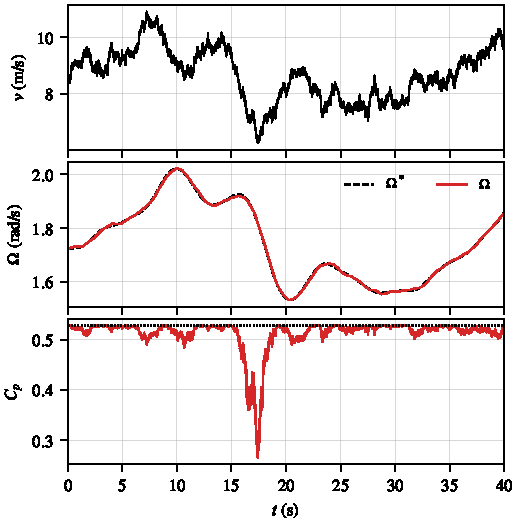
\includegraphics[width=\columnwidth]{mppt.pdf}
\caption{Robustness case, flat+PBC+ANN: wind speed, rotor speed and reference, and power coefficient
(dotted: $C_{p,\max}$ of the true turbine).}
\label{fig:mppt}
\end{figure}

\begin{figure}[t]
\centering
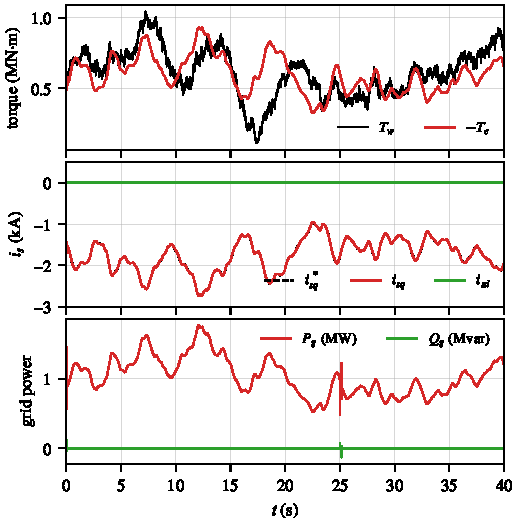
\includegraphics[width=\columnwidth]{machine.pdf}
\caption{Robustness case, flat+PBC+ANN: aerodynamic and electromagnetic torques, stator currents, and
grid active and reactive powers.}
\label{fig:machine}
\end{figure}

\begin{figure}[t]
\centering
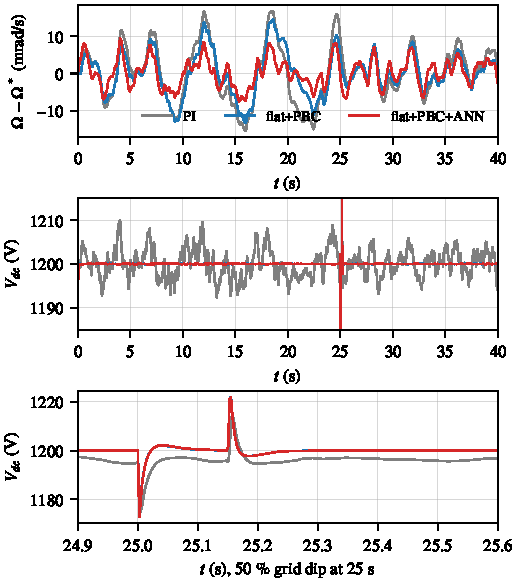
\includegraphics[width=\columnwidth]{comparison.pdf}
\caption{Robustness case: speed tracking error and DC-link voltage of the three controllers, and
DC-link voltage during the 50\,\% grid voltage dip.}
\label{fig:cmp}
\end{figure}

\begin{figure}[t]
\centering
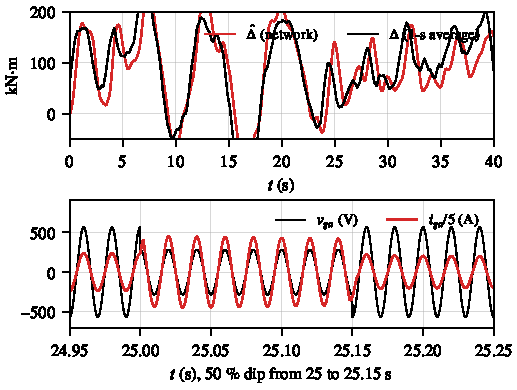
\includegraphics[width=\columnwidth]{grid.pdf}
\caption{Robustness case: network output $\hat\Delta$ and actual uncertainty $\Delta$ (aerodynamic model
and flux mismatch, 1-s average), and grid voltage and current of phase $a$ during the dip.}
\label{fig:grid}
\end{figure}

\subsection{Results}
Figs.~\ref{fig:mppt}--\ref{fig:grid} and Table~\ref{tab:res} summarize the results. The wind varies
between 6.2 and 10.9~m/s (Fig.~\ref{fig:mppt}). The rotor speed follows its reference; $C_p$
stays close to its maximum except during the fast wind decrease around 17~s, where the large inertia
prevents the rotor from slowing down quickly. The electromagnetic torque is negative and follows the
aerodynamic torque, $i_{sd}$ is kept at zero, and the grid power follows the captured power with
$Q_g=0$ (Fig.~\ref{fig:machine}).

\begin{table}[t]
\caption{Comparison of the Controllers (40 s, from $t=1$ s)}
\label{tab:res}
\centering
\footnotesize
\setlength{\tabcolsep}{3pt}
\begin{tabular}{lccc}
\toprule
Metric & PI & flat+PBC & flat+PBC+ANN\\
\midrule
\multicolumn{4}{l}{\emph{Nominal}}\\
IAE of $\Omega$ (rad) & 0.195 & 0.148 & 0.099\\
RMS error of $i_{sq}$ (A) & 0.057 & 0.044 & 0.042\\
Max $|V_{dc}-V_{dc}^*|$ (V) & 9.7 & 0.13 & 0.13\\
Energy to grid (kWh) & 10.255 & 10.259 & 10.253\\
MPPT efficiency (\%) & 97.7 & 97.7 & 97.7\\
Torque rate, std (MN$\cdot$m/s) & 0.166 & 0.178 & 0.194\\
\midrule
\multicolumn{4}{l}{\emph{Robustness}}\\
IAE of $\Omega$ (rad) & 0.237 & 0.179 & 0.117\\
RMS error of $i_{sq}$ (A) & 0.063 & 0.048 & 0.045\\
Max $|V_{dc}-V_{dc}^*|$, no dip (V) & 9.9 & 0.21 & 0.21\\
Max $|V_{dc}-V_{dc}^*|$, dip (V) & 24.9 & 26.0 & 27.2\\
Energy to grid (kWh) & 11.206 & 11.211 & 11.208\\
MPPT efficiency (\%) & 97.7 & 97.7 & 97.7\\
Torque rate, std (MN$\cdot$m/s) & 0.170 & 0.180 & 0.199\\
\bottomrule
\end{tabular}
\end{table}

\emph{Speed loop.} The feedforward of $J\dot\Omega^*$ and $\hat T_w$ in the flat law reduces the IAE of
the speed by 24\,\% (nominal) and 24\,\% (robustness) with respect to PI.
The network reduces it by a further 34\,\% and 35\,\%: it learns the mean
uncertainty $\Delta$, about 87~kN$\cdot$m in the robustness case (15\,\% of the
mean aerodynamic torque), within a few seconds, and follows its slow variations (Fig.~\ref{fig:grid}).
The price is a more active torque (11\,\% larger standard deviation of its rate). The captured
energy and the MPPT efficiency are almost identical for the three controllers: near the optimum, $C_p$ is
flat, so small speed errors have little effect on the energy.

\emph{DC link.} With the feedforward of $P_{dc}$, the flat law keeps $V_{dc}$ within
0.21~V of 1200~V outside the dip, against 9.9~V with the PI loop, which reacts
only to the voltage error. During the 50\,\% dip, the three controllers give a similar deviation of
about 26~V (2\,\% of $V_{dc}^*$), recovered within 50~ms (Fig.~\ref{fig:cmp}): it is set by the
current-loop dynamics, the GSC current doubling to keep the same power (Fig.~\ref{fig:grid}).

\emph{Currents.} The PBC and PI current loops have the same poles and both track the references with
errors below 0.1~A RMS for $i_{sq}$, i.e., less than 0.01\,\% of the rated current.

These results are obtained with the average converter model and an ideal PLL; the switching ripple,
the dead times and the PLL dynamics are not represented.

\section{Conclusion}
A 2~MW direct-drive PMSG wind energy conversion system was modeled in the receptor convention, with an
exact power balance that verifies the signs of the model. Its control combines flatness for the speed
and DC-link energy loops, passivity-based control for the current loops of both converters, and an RBF
network that learns the aerodynamic-torque and parameter uncertainty with a Lyapunov law. Under
turbulent wind and parameter mismatch, the flat structure reduces the speed tracking error with respect
to PI vector control and keeps the DC-link voltage almost constant thanks to its power feedforward; the
network further reduces the speed error at the price of a more active torque. The captured energy is
the same for all controllers. Future work will include a switched converter model, the PLL, pitch
control above rated wind and experimental validation.

\section*{Conflict of Interest}
The authors declare there are no conflicts of interest.

\begin{thebibliography}{99}
\bibitem{iea2024} International Energy Agency (IEA), \emph{World Energy Outlook 2024}, Paris, France, 2024.
\bibitem{gwec2024} Global Wind Energy Council (GWEC), \emph{Global Wind Report 2024}, Brussels, Belgium, 2024.
\bibitem{polinder2013} H. Polinder, J. A. Ferreira, B. B. Jensen, A. B. Abrahamsen, K. Atallah, and
R. A. McMahon, ``Trends in wind turbine generator systems,'' \emph{IEEE J. Emerg. Sel. Topics Power
Electron.}, vol.~1, no.~3, pp.~174--185, Sep. 2013.
\bibitem{wu2011} B. Wu, Y. Lang, N. Zargari, and S. Kouro, \emph{Power Conversion and Control of Wind
Energy Systems}. Hoboken, NJ, USA: Wiley-IEEE Press, 2011.
\bibitem{chinchilla2006} M. Chinchilla, S. Arnaltes, and J. C. Burgos, ``Control of permanent-magnet
generators applied to variable-speed wind-energy systems connected to the grid,'' \emph{IEEE Trans.
Energy Convers.}, vol.~21, no.~1, pp.~130--135, Mar. 2006.
\bibitem{yazdani2010} A. Yazdani and R. Iravani, \emph{Voltage-Sourced Converters in Power Systems:
Modeling, Control, and Applications}. Hoboken, NJ, USA: Wiley-IEEE Press, 2010.
\bibitem{mechter2016} A. Mechter, K. Kemih, and M. Ghanes, ``Backstepping control of a wind turbine for
low wind speeds,'' \emph{Nonlinear Dynamics}, vol.~84, no.~4, pp.~2435--2445, 2016.
\bibitem{messadi2015} M. Messadi, A. Mellit, K. Kemih, and M. Ghanes, ``Predictive control of a chaotic
permanent magnet synchronous generator in a wind turbine system,'' \emph{Chinese Phys. B}, vol.~24,
no.~1, Art.~no.~010502, 2015, doi: 10.1088/1674-1056/24/1/010502.
\bibitem{takhi2020} H. Takhi, K. Kemih, L. Moysis, \emph{et al.}, ``Passivity based control and
synchronization of perturbed uncertain chaotic systems and their microcontroller implementation,''
\emph{Int. J. Dyn. Control}, vol.~8, no.~3, pp.~973--990, 2020.
\bibitem{fliess1995} M. Fliess, J. L\'evine, P. Martin, and P. Rouchon, ``Flatness and defect of
non-linear systems: Introductory theory and examples,'' \emph{Int. J. Control}, vol.~61, no.~6,
pp.~1327--1361, 1995.
\bibitem{thounthong2010} P. Thounthong, S. Pierfederici, and B. Davat, ``Analysis of differential
flatness-based control for a fuel cell hybrid power source,'' \emph{IEEE Trans. Energy Convers.},
vol.~25, no.~3, pp.~909--920, Sep. 2010.
\bibitem{ortega1998} R. Ortega, A. Lor\'ia, P. J. Nicklasson, and H. Sira-Ram\'irez,
\emph{Passivity-Based Control of Euler-Lagrange Systems}. London, UK: Springer, 1998.
\bibitem{lewis1999} F. L. Lewis, S. Jagannathan, and A. Ye\c{s}ildirek, \emph{Neural Network Control of
Robot Manipulators and Nonlinear Systems}. London, UK: Taylor \& Francis, 1999.
\bibitem{regani2026} S. Regani, M. Messadi, and K. Kemih, ``A novel chaos control approach with
adaptive ANN compensation for a DFIG-based wind turbine,'' \emph{Mathematics}, under review, 2026.
\bibitem{hasan2021} S. M. M. Hasan and A. H. M. Shatil, ``Design and comparison of grid connected
permanent magnet synchronous generator non-salient pole and salient pole rotor wind turbine,''
\emph{AIUB J. Sci. Eng.}, vol.~20, no.~2, pp.~40--46, 2021.
\bibitem{heier2014} S. Heier, \emph{Grid Integration of Wind Energy: Onshore and Offshore Conversion
Systems}, 3rd ed. Chichester, UK: Wiley, 2014.
\bibitem{khalil2002} H. K. Khalil, \emph{Nonlinear Systems}, 3rd ed. Upper Saddle River, NJ, USA:
Prentice Hall, 2002.
\end{thebibliography}

\end{document}
